\chapter{引言}

\section{项目背景}
在线评测(Online Judge,下文简称为OJ)系统是用于编程练习的平台,用户可以在平台上搜索相关的编程题目,并在线提交自己的答案(即C、Python、JavaScript等语言的源代码)。OJ系统会对这些源代码进行编译和执行,并通过预先设计的测试数据来评测程序源代码的正确性,最后将评测结果呈现给用户。

OJ系统最初使用于ACM-ICPC国际大学生程序设计竞赛和OI信息学奥林匹克竞赛中的自动判题和排名。现广泛应用于世界各地高校学生程序设计的训练、参赛队员的训练和选拔、各种程序设计竞赛以及数据结构和算法的学习和作业的自动提交判断中。北航软件学院的AC编程平台就是一个传统的OJ系统,程序设计基础、大学计算机基础等北航校内的课程都依托于AC编程平台开展。

但是,传统的OJ系统仍然存在着许多局限性:它通常以黑盒测试的形式判定程序的正确性,简单地给用户呈现通过的测试用例的数量,不检查用户的代码质量。它通常也仅能对单文件的源代码进行评测,不能对多文件的项目进行评测。目前市面上虽然有极少数的OJ系统(如北航编译原理课程使用的rurikawa系统)支持多文件的评测,但这些OJ系统不能支撑有一定并发量的评测。当遇到多个用户同时评测的情况时,这些OJ系统的评测队列会非常拥挤,用户需要等待极长的时间才能获得评测的结果。另外,传统的OJ平台太过纯粹了,用户只能在OJ平台上验证已知的知识,而新知识的获取则需另寻他途,用户经常需要在互联网的海洋中搜索许久才能领会到某个编程练习的背景知识。

\begin{figure}[H]
    \centering
    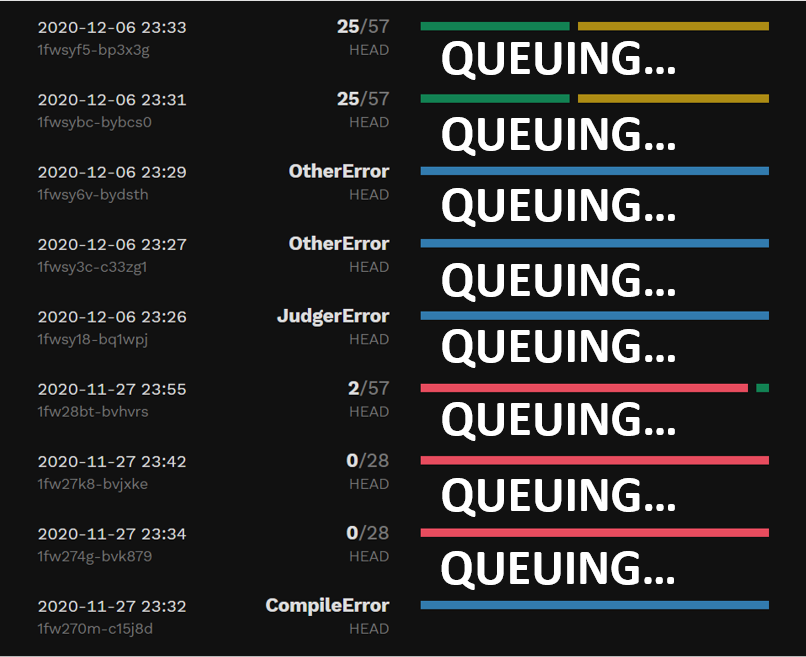
\includegraphics[width=0.7\textwidth]{figure/queuing.png}
    \caption{\textbf{传统OJ系统拥挤的评测队列}}
    \label{fig:queuing}
\end{figure}

\section{项目概述}

PhoeniX是一体化的编程学习平台,旨在为编程学习的相关课程以及编程学习者提供服务。在PhoeniX平台上,用户可以搜索并查阅特定方向的教程和题目,选择题目进行练习并检测自己编写的程序的正确性。用户可以自发地成立组织,在组织内进行教程与题目的发布、共享相关资源、举办范围性的比赛、进行相关讨论……PhoeniX还能基于用户的评测结果以及大数据的统计分析结果,给用户推荐合适的教程与题目,帮助用户提高技术水平与编程能力。

相比于传统的OJ平台,PhoeniX支持对多文件的项目进行评测,打破了传统OJ平台单文件评测的限制,解决了人工手动运行、评测项目级代码的痛点问题。PhoeniX还创新性地将评测过程转移到了用户端,有效降低了用户的评测等待时间,同时大幅减少了远程服务器的资源消耗,可以良好地应对各种大型比赛活动的评测需求,非常适合成本有限的课堂教学环境。另外,PhoeniX还解决了传统OJ平台的内容过于纯粹的问题,PhoeniX在题目评测的基础上加入了资源共享、轻社交、交互式教程等元素,提供了完整的的编程学习服务。

\section{项目创新点与先进性}

\begin{enumerate}
    \item 将传统OJ平台的评测过程转移到用户端进行,采用分布式评测的思想,极大地减少了用户评测的等待时间,提高了用户体验。
    \item 基于Electron框架开发,支持跨平台使用。PhoeniX项目的客户端在Windows、Linux和Mac OS等操作系统上均可使用,全平台数据互通。
    \item 支持对含有多文件、具有复杂目录结构的项目进行评测,在理论上能够支持几乎所有类型的项目评测,打破了传统OJ的单文件评测限制。
    \item 支持对Java、Python、JavaScript、C++、Golang等多语言的评测。可以自定义配置编译和运行的命令,以支持任何编程语言。
    \item 用户可以自行发布题目和教程。PhoeniX允许用户使用Markdown语法与Latex语法进行题目与教程的编写,支持嵌入可交互式的代码执行环境。
    \item 提供组织管理功能,用户可以自行创建组织。在组织内,用户可以开展比赛、在组织论坛内进行讨论、共享组织的题目与教程。
    \item 提供教程和题目的智能推荐,PhoeniX可以给用户推荐最适合用户的题目和教程,提高用户的学习体验。
\end{enumerate}

\section{项目难点与解决方案}

\begin{enumerate}
    \item 如何在用户机上向目标程序调用编译、执行的相关命令?\\
          利用Node.js的相关多进程API创建子进程,父子进程之间采用管道通信。
    \item 如何将输入数据传给目标程序,并获取到目标程序的输出?\\
          将子进程的输入输出进行重定向,将用户程序的输出转存到文件中。
    \item 如何在支持Markdown语法的同时,渲染代码的可执行环境?\\
          使用markdown-it渲染器作为Markdown文本的基础渲染器,并编写相关插件嵌入Visual Studio Code类似风格的代码执行环境。
    \item 如何判断用户程序已执行超时?\\
          利用Node.js的相关多进程API,设定子进程的运行时间限制,当到达限定时间时子进程返回特定的退出码。
    \item 如何实现PhoeniX的跨平台构建?\\
          在CI/CD工作流中将构建分为Windows构建、Linux构建、Mac OS构建三个任务,利用Github Actions进行自动构建。
\end{enumerate}